\section{~Wave Model Structure and Data Flow} \label{chapt:run}
\newcounters

\input{run/design}
\input{run/core}
\input{run/das}
\vssub
\subsection{~Auxiliary programs} \label{sec:auxprog}
\vsssub
\subsubsection{General concepts}
\vsssub

All auxiliary programs presented here, with the exception of the track output
post-processor, read input from a pre-defined input file. The first character
on the first line of the input file will be considered to be the comment
character, identifying comment lines in the input file. This comment character
has to appear on the first position of input lines to be effective. In all
examples in the following sections lines starting with '{\tt \$}' therefore
only contain comment. The programs furthermore all write formatted output to
the standard output unit.

In the following sections, all available auxiliary programs are described
using an example input file with all options included (partially as
comment). These files are identical to the distributed example input
files. The sections furthermore show the name of the executable program, the
program name (as appears in the program statement), the source code file and
input and output files and their unit numbers (in brackets behind the file
name). Input and output files marked with \opt are optional. The intermediate
files mentioned below are all {\F unformatted}, and are not described in
detail here. Each file is written and read by a single routine, to which
reference is made for additional documentation.

\begin{list}{}{\itemsep 0mm \parsep 0mm \leftmargin 40mm \labelwidth 30mm}
\item[{mod\_def.ww3} \hfill] Subroutine {\F w3iogr} ({\file w3iogrmd.ftn}).
\item[{out\_grd.ww3} \hfill] Subroutine {\F w3iogo} ({\file w3iogomd.ftn}).
\item[{out\_pnt.ww3} \hfill] Subroutine {\F w3iopo} ({\file w3iopomd.ftn}).
\item[{track\_o.ww3} \hfill] Subroutine {\F w3iotr} ({\file w3iotrmd.ftn}).
\item[{restart.ww3}  \hfill] Subroutine {\F w3iors} ({\file w3iorsmd.ftn}).
\item[{nest.ww3}     \hfill] Subroutine {\F w3iobc} ({\file w3iobcmd.ftn}).
\item[{partition.ww3}\hfill] Subroutine {\F w3iosf} ({\file w3iosfmd.ftn}).
\end{list}

\noindent
Preprocessing and compilation of the programs is discussed in the following
two chapters. Examples of test runs of the model are provided with the source
code.

\pb

\input{run/ww3_grid.tex}
\input{run/ww3_strt.tex}
\input{run/ww3_bound.tex}
\input{run/ww3_bounc.tex}
\input{run/ww3_prep.tex}
\input{run/ww3_prnc.tex}
\input{run/ww3_prtide.tex}
\input{run/ww3_shel.tex}
\input{run/ww3_gspl.tex}
\input{run/ww3_multi.tex}
\vsssub
\subsubsection{Grid Integration} \label{sub:ww3gint}
\vsssub
\proddefH{ww3\_gint}{w3gint}{ww3\_gint.ftn}
\proddeff{Input}{ww3\_gint.inp}{Formatted input file for program.}{10}
\proddefa{mod\_def.*}{Model definition files in \ws\ format for base and target grids}{20}
\proddefa{out\_grd.*}{Gridded field files in \ws\ format for base grids}{30+}
\proddeff{Output}{standard out}{Formatted output of program.}{6}
\proddefa{out\_grd.*}{Gridded field files in \ws\ format for target grid}{30+}

\vspace{\baselineskip}
\noindent
This post processor program takes field data from several overlapping grids
and produces a unified output file. The different model definition and field
output files are identified by the unique identifier associated with each
specific grid. At this moment the program works with curvilinear and
rectilinear grids. A weights file {\file WHTGRIDINT.bin} is written 
that can be read in subsequent runs using identical origin-destination grids, 
saving substantial time in cases using large number of input grids and/or 
high-resolution target grids.

\inpfile{ww3_gint.tex}

\vspace{\baselineskip}
\vspace{\baselineskip}
\noindent
Note that this program can be used in concert with the grid splitting program
{\file ww3\_gspl}, and that {\file ww3\_gspl.sh} has an option to produce a
template input file for his program (see \para\ref{sub:ww3gspl}).

\pb

\input{run/ww3_outf.tex}
\input{run/ww3_ounf.tex}
\input{run/gx_outf.tex}
\input{run/ww3_grib.tex}
\input{run/ww3_outp.tex}
\input{run/ww3_ounp.tex}
\input{run/gx_outp.tex}
\input{run/ww3_trck.tex}
\input{run/ww3_systrk.tex}
\vsssub
\subsubsection{The Restart File Processor} \label{sec:ww3uprstr}
\vsssub

\proddefH{ww3\_uprstr}{ww3uprstr}{ww3\_uprstr.ftn}
\proddeff{Input}{ww3\_uprstr.inp}{Input file for restart file
post-processor.}{10}
\proddefa{mod\_def.ww3}{Model definition file.}{20}
\proddefa{restart.ww3}{Restart File}{-}
\proddefa{XXXX.grbtxt}{SWH Analysis file in grbtxt format.}{10}
\proddeff{Output}{restart001.ww3}{Updated restart file.}{-}

\inpfile{ww3_uprstr.tex}

\vspace{\baselineskip} 

\paragraph{Introduction \newline } 

The majority of the observations for the sea surface wave field is 
observations of the diagnostic variable: Significant Wave Height (SWH). 
Therefore, the wave data assimilation (WDA) often happens in the SWH 
space and subsequently this  information has to be transfered to the 
prognostic space, wave spectrum (WS) to be imposed as boundary and/or 
initial condition (BIC). 

\subparagraph{Purpose of the \textbf{ww3\_uprstr} } Redistribution of 
the energy from the analysis of the SWH field to the field of WS as 
they have been saved at the restart file.

\subparagraph{Core algorithm \newline } 
The \textbf{ww3\_uprstr} sets the SWH of the background spectrum equal to 
the SWH of the analysis and modifies the shape of the spectrum according 
to the user's prescibed spectrum shape. The \textbf{ww3\_uprstr} has been  
implemented as an extension of the restart reader and it requires as inputs: 
the restart file, the SWH of the analysis, and the \textbf{ww3\_uprstr.inp} 
(see above) with the user's defined options; additional files may be
required.

\paragraph{How to Use the ww3\_uprstr \newline}
To use the \textbf{ww3\_uprstr}, the users have to follow the same logic 
as for all the WAVEWATCH III programs. In summary: 

\begin{enumerate}
   \item \textbf{Download the source code} \newline
   The \textbf{ww3\_uprstr} source code is included to the official WAVEWATCH III
   release, starting with the version 6.03.
   \item \textbf{Compile the code} \newline
   The \textbf{ww3\_uprstr} is compiled the same way as all the auxiliary programs 
   of WAVEWATCH III, see the appropriate section of the manual. For debugging outputs, 
   use the  \textbf{T} flag at the switch file.
   \item \textbf{Run the ww3\_uprstr} \newline
   Description of steps to run the \textbf{ww3\_uprstr}:
   \begin {description}
      \item{Required Input files: \newline}
      \begin{itemize}
         \item \textbf{Restart file.} This file has been created by WW3 during the warmup run
         of the model or during the previous cycle.
         Expected filename: \textbf{restart.ww3}.
         \item \textbf{mod\_def.ww3}
         \item \textbf{ww3\_uprstr.inp.} This is the input file for the \textbf{ww3\_uprstr}. 
         The users have to define i. the date of the assimilation, ii. the method of energy
         redistribution and iii. depending on the method: a percentage or an inputfile.
         \item \textbf{Input file of analysis.} The file can have any name, but the suffix 
         defines the reader used for importing the data. Currently, the reader supports only
         \textbf{grbtxt} format. This is a text file created with wgrib2 from the grib2 file 
         of the analysis and it has the following structure:\newline

         \begin{tabular}{|c|}
            \hline
            NX NY       \\
            VAL0001     \\
            VAL0002     \\
            ...         \\
            VAL(NX*NY)  \\
            \hline   
          \end{tabular}
    \newline
    \item To run the executable: \newline 
          \textgreater \$EXE/ww3\_uprstr \newline 
          If all the inputs are correctly prepared, a new restart file, 
          (\textbf{restart001.ww3}), will be created. The \textbf{ww3\_uprstr} 
          exports the updated spectra in the same format as the restart.ww3. 
          To be applied as BIC for the initialization of the next prediction cycle,
          it has to be renamed: \newline
          \textgreater mv \textbf{restart001.ww3} \textbf{restart.ww3}) \newline      
          The updated restart file is used as normally.
      \end{itemize}
   \end{description}
   
   \fbox{
      \parbox{\linewidth}{
         \textbf{Tips}
         \begin{itemize}
            \item The restart file has to be created with the same WW3 version as 
         the \textbf{ww3\_uprstr}; there is not backwards compatibility.
            \item The starting time of the assimilation defined at \textbf{ww3\_uprstr.inp}
         has to be the same with the time at the restart file.
         \end{itemize}
         }
   }
\end{enumerate}
 
\subparagraph{Update method \newline}
The users have to define the update algorithm of their choice at the
\textbf{ww3\_uprstr.inp}. The options for updating the restart file are defined at the 
ww3\_uprstr.inp with the flag UPD[N], where N could be 0F, 0C, 1, 2,... 
For UPDN, with N \textless 2, the same correction is applied to the whole grid;
Expected input: PRCNTG, as defined at fac.
For UPDN, with N \textgreater 1 each gridpoint has its own update factor and the input
is at grb2txt format. For more details about the current implementation see the 
~\ref{fig:uprstrflowchart}.

\begin{figure} \begin{center}
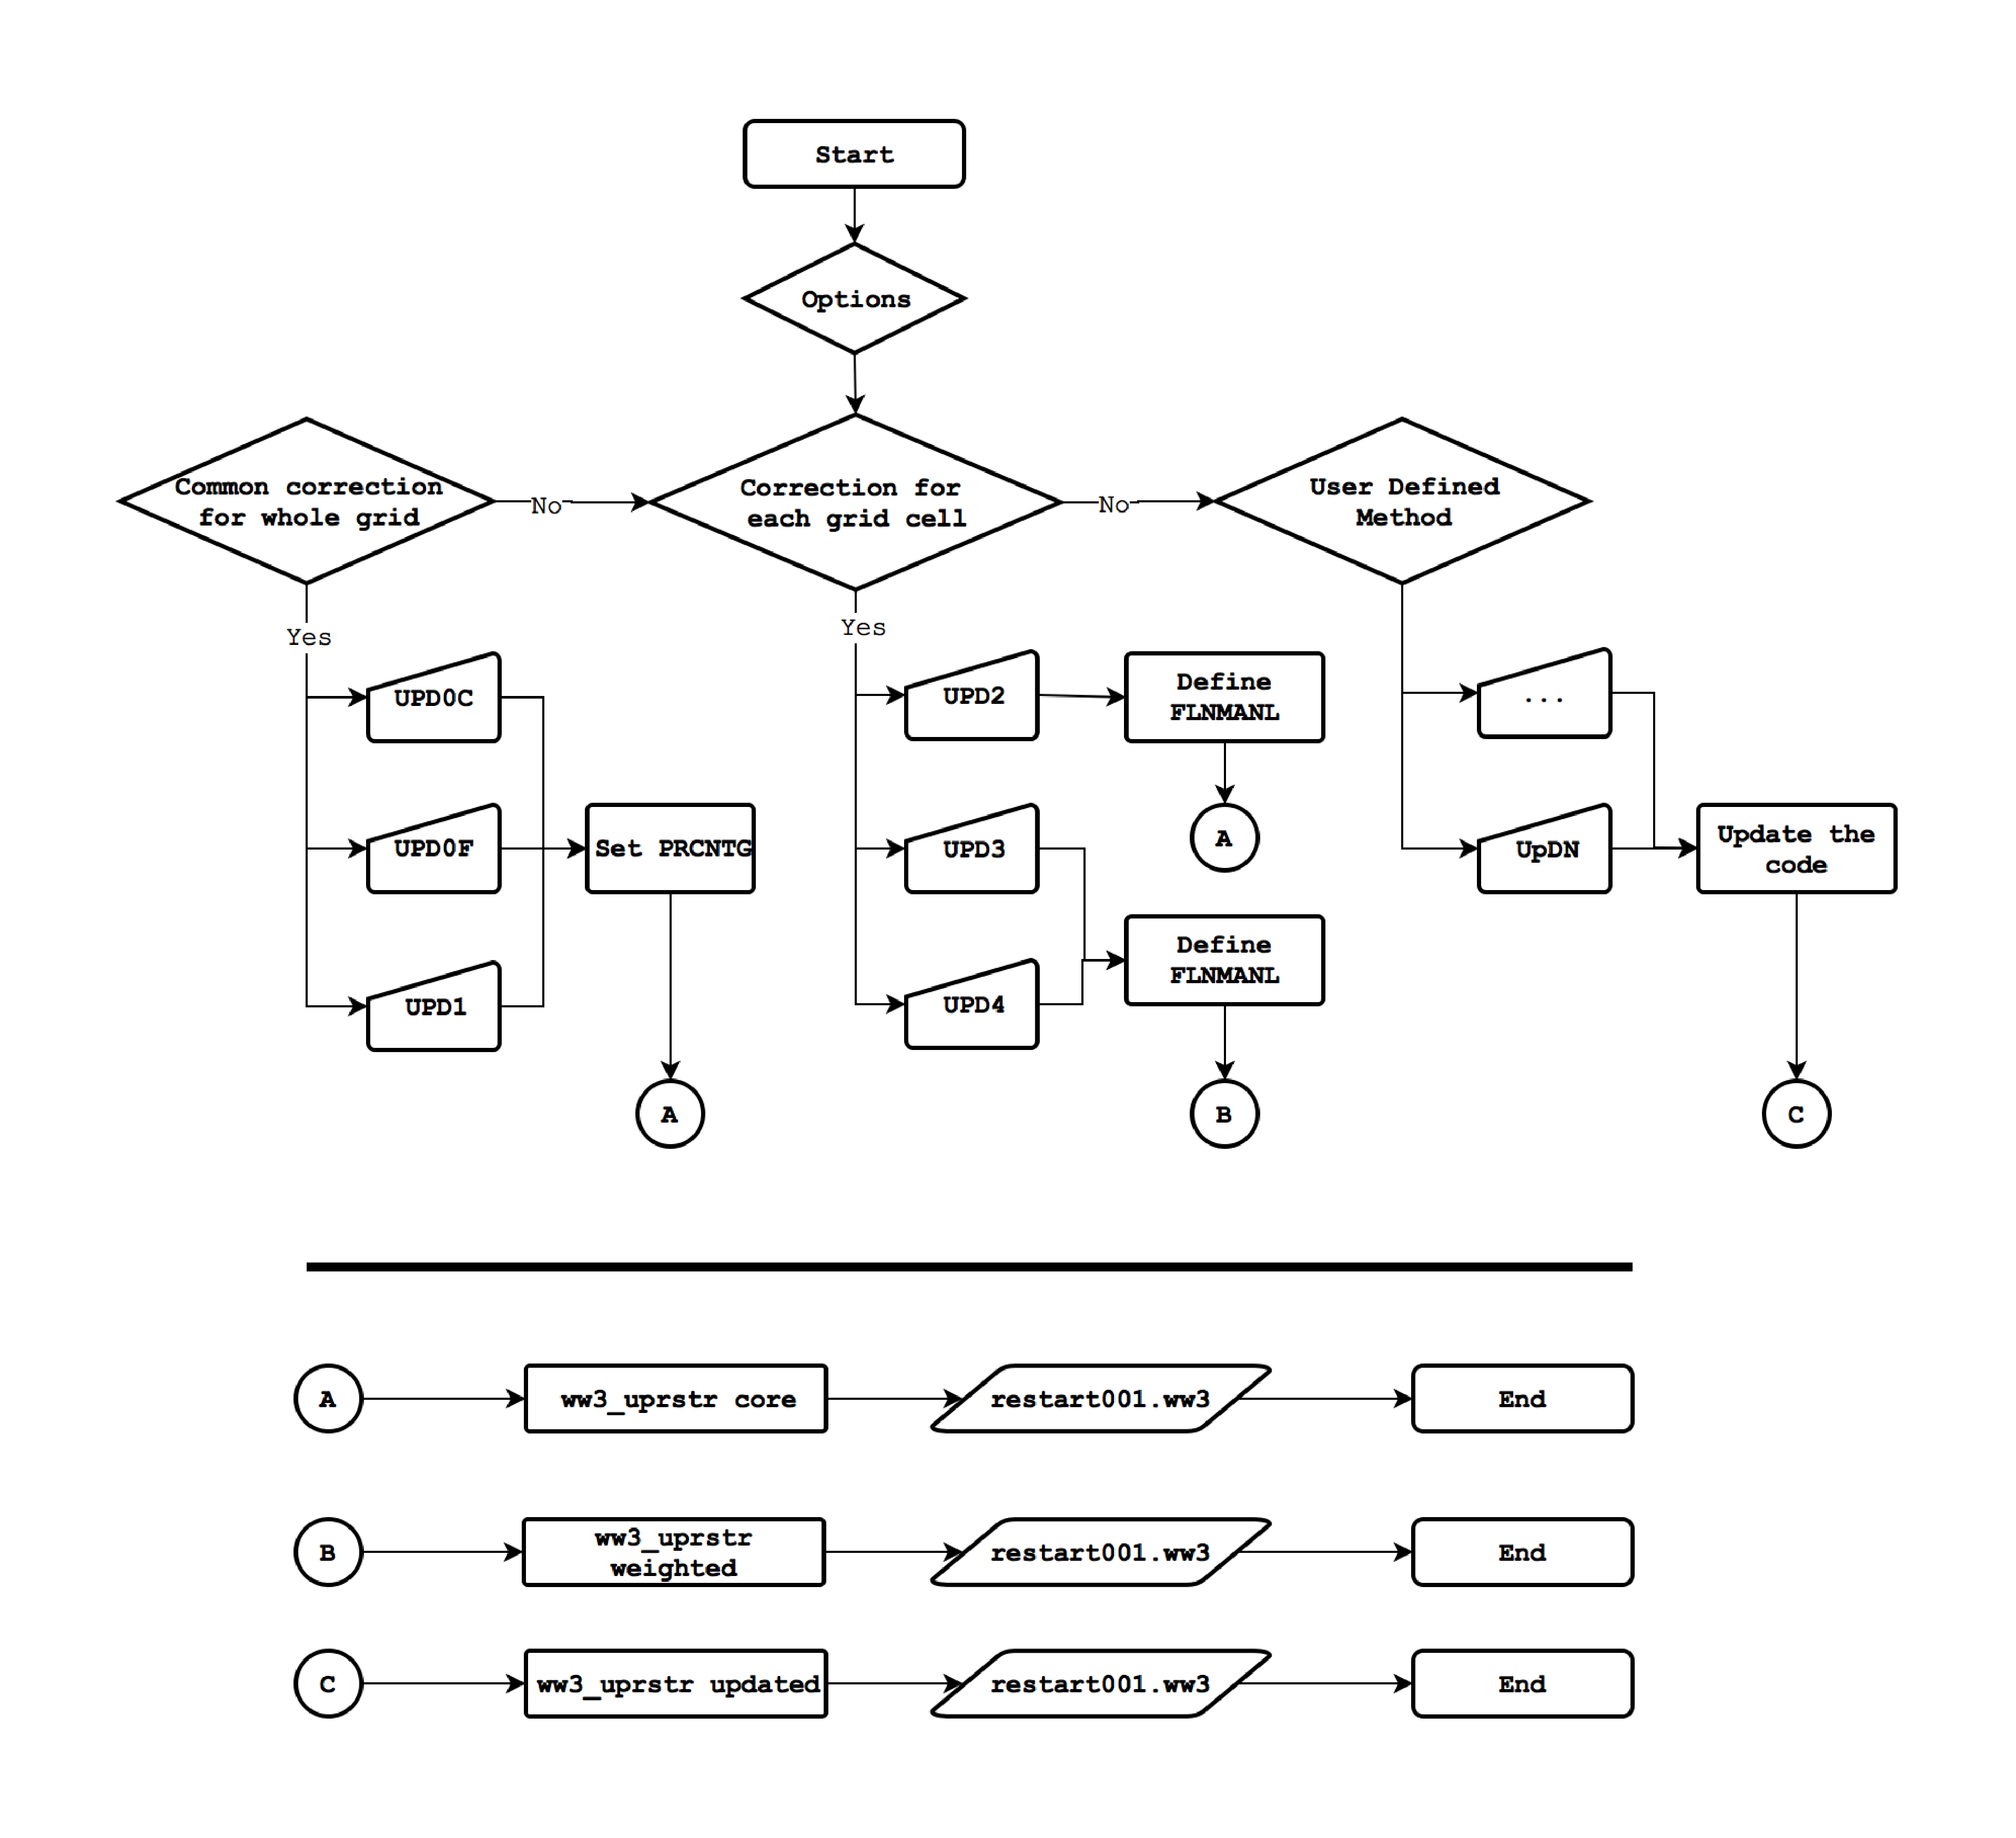
\includegraphics[width=0.9\textwidth]{./run/uprstr.eps}
\caption{Flowchart of the implemented methods for updating the wave spectra at the WW3 
restart file. Additional methods can be implemented by adding UPD options to the namelist.}
\label{fig:uprstrflowchart} \botline
\end{center}
\end{figure}

The following UPD options are available:
\begin{enumerate} 
   \item UPD0C:: Option 0C  All the spectra are updated with a constant 
      fac=(SWH\_Bckg-SWH\_Anl)/SWH\_Anl.
   \item UPD0F:: Option 0F  All the spectra are updated with a constant 
      fac=SWH\_Anl/SWH\_Bckg. 
   \item UPD1 :: Option 1   The fac(x,y,frq,theta), is weighted according to
      the \% of energy at each spectral bin; fac the same as UPDOF.
   \item UPD2 :: Option 2   The fac(x,y,frq,theta), is calculated at 
         each grid point according to SWH\_Bckg and SWH\_Anl
   \item UPD3 :: Option 3   The update factor is a surface with the shape of 
      the background spectrum. 
   \item UPD4 :: [NOT INCLUDED in the current version, just keeping the spot]
      Option 4  The generalization of the UPD3. The update factor is the sum of surfaces 
      which are applied on the background spectrum 
\end{enumerate}

Any additional method for the redistribution of the energy to the WS could be added 
by adding a new entry at the namelist of the \textbf{ww3\_uprstr.inp}.

\subparagraph{Example \newline}
In this section, an example of the simplest WDA application is discussed.
The figure ~\ref{fig:waveDAflowchart} shows how the \textbf{ww3\_uprstr} 
is used in the framework of a simple wave analysis system. \newline

A WW3 run (from the previous cycle or from the warm up of the model) provides the
background field of SWH and the corresponding restart file at the appropriate time. 
The format of the background SWH field has to be compatible with the WDA module inputs.

The WDA module uses the background field and the available observations
for the time of analysis, produces the analysis (\textbf{XXXX.grbtxt}) and exports 
the field of SWH in grbtxt format.

The analysis file, the mod\_def.ww3, the restart.ww3 file and the ww3\_uprstr.inp 
are the input files for the \textbf{ww3\_uprstr}. If all the options and input 
files are correctly prepared, it takes approxmately one minute to update a grid 
of 260000 grid nodes and generate the output on a single processor. 
The updated restart file has to be renamed, at the expected file name, in the case of this
example restart.ww3. \newline  

   \fbox{
      \parbox{\textwidth}{
      \textbf{Note: }
      All \ncep's WDA systems use GRIB2 format, thereore there is always an intermediate
      step to transfer the grib files to the appropriate format. The used software is WGRIB2 
      and more information can be retrieve from the 
      \href{http://www.cpc.ncep.noaa.gov/products/wesley/wgrib2} {official website}.       
      }
   }

\begin{figure} \begin{center}
\includegraphics[width=0.9\textwidth]{./run/waveDA.eps}
\caption{Flowchart of simplified wave data assimilation system, 
showing the role of the {ww3\_uprstr}, the required input files,
and the resulted output of the updated restart file.}
\label{fig:waveDAflowchart} \botline
\end{center}
\end{figure}

%\paragraph{How to Update the ww3\_uprstr \newline}
%Add data readers, mainly for machine independent binary data and wgrib2.

\pb


% tab:fields

\begin{table} \begin{center}
\begin{tabular}{|c|c|c|c|c|c|} \hline
group & field & description                  &  file        & GRIB1 & GRIB2   \\
      &                              &  extension   & data  & data    \\ \hline \hline
 1 & 1 & depth                           & {\file .dpt} &  --  &    --    \\
 1 & 2 & mean current components         & {\file .cur} &  --  &    --    \\
 1 & 3 & wind speed                      & {\file .wnd} &  32  &  0,2,1   \\
   &&  wind direction                 &              &  31  &  0,2,0   \\
   &&  wind $u$                       &              &  33  &  0,2,2   \\
   &&  wind $v$                       &              &  34  &  0,2,3   \\
 1 & 4 & air-sea temp. dif.              & {\file .dt}  &  --  &    --    \\
 1 & 5 & water level                     & {\file .wlv} &  --  &  10,3,1  \\
 1 & 6 & ice coverage                    & {\file .ice} &  91  &  10,2,0  \\
 2 & 1 & wave height $H_s$               & {\file .hs}  & 100  &  10,0,3  \\
 2 & 2 & mean wave length                & {\file .l}   &  --  &    --    \\
 2 & 3 & mean wave period $T_{m0,2}$     & {\file .t02} &  --  &    --    \\
 2 & 4 & mean wave period $T_{m0,1}$     & {\file .t}   & 103  &  10,0,15 \\
 2 & 5 & mean wave period $T_{m0,-1}$    & {\file .tm1} &  --  &    --    \\
 2 & 6 & peak frequency $f_p$            & {\file .fp}  & 108  &  10,0,11 \\
 2 & 7 & mean wave direction $\theta_m$  & {\file .dir} & 101  &    --    \\
 2 & 8 & directional spread $\sigma$     & {\file .spr} &  --  &    --    \\
 2 & 9 & peak direction $\theta_p$       & {\file .dp}  & 107  &  10,0,10 \\
 4 & 1 & $H_s$ of partition              & {\file .phs} & 102,105 & 10,0,5/8 \\
 4 & 2 & $T_p$ of partition              & {\file .ptp} & 110,106 & 10,0,6/9\\
 4 & 3 & $L_p$ of partition              & {\file .plp} &  --  &    --    \\
 4 & 4 & $\theta_m$ of partition         & {\file .pdir} & 109,104 & 10,0,4/7 \\
 4 & 5 & $\sigma$ of partition           & {\file .psi} &  --  &    --    \\
 4 & 6 & wind sea fraction of part.      & {\file .pws} &  --  &    --    \\
 4 & 7 & total wind sea fraction         & {\file .wsf} &  --  &    --    \\
 4 & 8 & number of partitions            & {\file .pnr} &  --  &    --    \\
 5 & 1 & friction velocity comp.         & {\file .ust} &  --  &    --    \\
 5 & 2 & Charnock parameter for air side & {\file .cha} &  --  &    --    \\
 5 & 3 & Energy flux $\int C_g E(f) df$  & {\file .CgE} &  --  &    --    \\
 5 & 4 & Wind to wave energy flux        & {\file .faw} &  --  &    --    \\
 5 & 5 & Wave-supported stress           & {\file .taw} &  --  &    --    \\
 5 & 6 & Upward wave-supported stress    & {\file .twa} &  --  &    --    \\
 5 & 7 & Whitecap coeverage              & {\file .wcc} &  --  &    --    \\
 5 & 8 & Average whitecap foam thickness & {\file .wcf} &  --  &    --    \\
 5 & 9 & Significant breaking wave height& {\file .wch} &  --  &    --    \\
 5 & 10 & Whitecap moment                 & {\file .wcm} &  --  &    --    \\ \hline
\end{tabular} \end{center}
\caption{~Field output post processors ancillary data.} \label{tab:fields}
\vspace{0.5in}
\end{table}

\begin{table} \begin{center}
\begin{tabular}{|c|c|c|c|c|c|} \hline
group & field & description                  &  file        & GRIB1 & GRIB2   \\
      &                              &  extension   & data  & data    \\ \hline \hline
 6 & 1 & radiation stress                & {\file .Sxy} &  --  &    --    \\
 6 & 2 & Breaking wave momentum flux     & {\file .two} &  --  &    --    \\
 6 & 3 & Bernoulli head                  & {\file .J} &  --  &    --    \\
 6 & 4 & Breaking wave energy flux       & {\file .foc} &  --  &    --    \\
 6 & 5 & Stokes transport                & {\file .tus} &  --  &    --    \\
 6 & 6 & Surface Stokes drift            & {\file .uss} &  --  &    --    \\
 6 & 7 & Second order pressure at $k=0$  & {\file .p2s} &  --  &    --    \\
 7 & 1 & near-bottom amplitude           & {\file .cfd} &  --  &    --    \\
 7 & 2 & near-bottom velocity            & {\file .ubr} &  --  &    --    \\
 7 & 3 & bedform parameters              & {\file .bed} &  --  &    --    \\
 7 & 4 & Energy flux to bot. boundary layer & {\file .fbb} &  --  &    --    \\
 7 & 5 & Momentum flux to bot. boundary layer & {\file .tbb} &  --  &    --    \\
 8 & 1& mean square slopes              & {\file .mss} &  --  &    --    \\
 8 & 2 & Phillips constant               & {\file .msc} &  --  &    --    \\
 9 & 1 & average time step               & {\file .dtd} &  --  &    --    \\
 9 & 2 & cut-off frequency $f_c$         & {\file .fc}  &  --  &    --    \\
 9 & 3 & cut-off frequency $f_c$         & {\file .fc}  &  --  &    --    \\
 9 & 4 & maximum CFL for X-Y advection   & {\file .cfx} &  --  &    --    \\
 9 & 5 & maximum CFL for $\theta$ advection & {\file .cfd} &  --  &    --    \\
 9 & 6 & maximum CFL for $k$ advection   & {\file .cfk} &  --  &    --    \\
 10 & 1 & user defined \#1                & {\file .us1} &  --  &    --    \\
 10 & 2 & user defined \#2                & {\file .us2} &  --  &    --    \\ \hline
%13 & wind sea period $T_w$           & {\file .fpl} & 110  &    --    \\
%14 & wind sea direction $\theta_w$   & {\file .dpl} & 109  &    --    \\

\end{tabular} \end{center}
\caption*{Table~\ref{tab:fields}, continued.} 
\vspace{0.5in}
\end{table}

\clearpage

%\bpage
